\documentclass{article}
\usepackage{times}
\usepackage{amsmath}
\usepackage{amssymb}
\usepackage{algorithmic}
\usepackage[ruled,linesnumbered,noend,oldcommands]{algorithm2e}
\usepackage[T1,hyphens]{url}
\usepackage{xspace}
\usepackage{graphicx}
\usepackage{listings}
\lstset { %
    language=C++,
    %backgroundcolor=\color{black!5}, % set backgroundcolor
    basicstyle=\footnotesize,% basic font setting
}

\begin{document}

\begin{abstract}
\end{abstract}

\section{Introduction}
The vast majority of modern SAT solvers used in industrial applications are based on the conflict-driven clause learning (CDCL) algorithm. In a CDCL SAT solver, backtracking occurs after every conflict, where all literals from one or more decision levels become unassigned, before the solver resumes making decisions and performing unit propagations. It turns out that many of the literals that are unassigned during a backtrack will often be re-assigned again in roughly the same order when the solver continues. This results in many of the exact same propagation steps being repeated over and over again during the execution of the solver, and avoiding these repetitions could result in a significant speedup.

Chronological backtracking \cite{DBLP:conf/lpar/2013, DBLP:conf/sat/MohleB19, DBLP:conf/sat/NadelR18} addresses this inefficiency by heuristically backtracking fewer levels up the trail after learning a clause. However, chronological backtracking breaks some traditional invariants of the SAT solver, namely that literals are supposed to appear on the trail in monotonically increasing order by decision level, and can be complex to implement. Additionally, it does not allow the search to have as much flexibility in deciding the order of literals to assign, since leaving a large portion of the trail intact "in a sense" forces decisions originally used to construct that portion. Some empirical evidence also suggests that it is only beneficial when used sparingly (e.g., when the number of levels to be backtracked over is greater than 100).

We propose an alternative method, "trail saving", where we cache the part of the trail that is unassigned during a backtrack and then attempt to restore implied parts of it as each new decision is made. Trail saving preserves the traditional invariants of the SAT solver and its basic version is very simple to implement. It also allows the search to choose the order of decisions, but helps make propagation faster. We explore the theoretical speedup that trail saving provides, develop some enhancements to make the idea more effective, and demonstrate experimentally that it speeds up state-of-the-art SAT solvers by a non-trivial factor.

\section{Background}
We will assume the reader is familiar with SAT solving and the basics of the CDCL algorithm \cite{DBLP:series/faia/SilvaLM09}. We will use the notion of a trail to represent a sequence of literals corresponding to the current partial assignment. The literals appear on the trail in the order in which they were assigned. Associated with every literal on the trail is a decision level. Decision level 0 represents all literals which are implied by the formula itself and subsequent decisions start the beginning of a new decision level. When a literal is made true by unit propagation, the literal is given its decision level and a reason clause, where the reason clause is the clause that was made unit by propagation in order to imply this literal. Most modern solvers use the two-literal watch scheme to make unit propagation more efficient.

\section{Trail Saving}
It can be observed that a SAT solver often repeats the same propagations over and over again during execution. Although no two descents down the trail will ever be identical because of clause learning, the solver will often propagate many of the same literals with the same reasons in a similar order to what it had done previously, especially since the order of the decisions usually remains similar. We plan to cache the part of the trail that we are backtracking over and use it to restore some of those literals without propagating them from scratch.

\subsection{Storing the trail cache}
The first step that is needed to use "trail saving" is to store the literals which are being unassigned during a backtrack, along with their respective reason clauses, in a "trail cache". Decisions should be marked with a null reason. The literals should appear in the same order on the trail cache as they had appeared on the trail. We will adopt the notation that the "top" of the trail cache is initially set to be the literal that appeared the earliest on the trail and will get updated as the trail cache gets used up. Note that initially the top of the trail cache is always a decison (i.e., the start of a new decision level). As the literals from the trail cache get restored (i.e., assigned), the top of the trail cache points to the next literal not yet restored.

\subsection{Restoring the trail cache}
We will base trail saving on a convenient observation. If the top of the trail cache becomes true at any point, every literal after the top of the trail cache up until the next decision literal (i.e., the next literal with a null reason) is implied by the current trail. The top of the trail cache can become true either by decision or unit propagation, and this observation still holds.\newline

\textit{Proof} Let $L_0$ be the set of literals on the trail after backtracking, $L_1$ be the set of literals on the current trail, and $L_c[i]$ denote the set of the first i literals on the trail cache. The $i$th literal on the trail cache is implied by $L_0 \cup L_c[i-1]$, as long as the $i$th literal was not a decision. $L_0 \subseteq L_1$, since $L_1$ starts out as $L_0$ and adds non-contradictory literals (by decision or unit propagation). Therefore, the $i$th literal on the trail cache is implied by $L_1 \cup L_c[i-1]$. Assume the top of the trail cache is true. Then, from above, every literal up until the next decision would be implied. $\blacksquare$\newline

Once the backtrack has been completed and the solver resumes with decisions and propagations, we will attempt to restore parts of the trail cache automatically during propagation to make it faster. When a literal is to be propagated, we first check the top of the trail cache to determine its truth value. If that literal's truth value is true, we assign all of the literals that come after it on the trail cache to be true up until (and excluding) the next the next literal with a null reason. If at any time the top of the trail cache is a literal with a non-null reason whose truth value is already false, we determine a conflict has occurred with the conflict clause being that literal's reason. At the beginning of a new backtrack, the trail cache is cleared and a new trail cache is generated.

A potentially quadratic speedup can be realized during the propagation of these literals since they are being propagated as a set, rather than one at a time. We will illustrate this with an example.\newline

\textit{Example 1} Suppose the literals $x_1, ... x_n$ are on the trail cache, with none of them having a null reason, and $x_1$ becomes true (e.g., the solver makes a decision for $x_1$ to be true). Then, $x_2, ... x_n$ are implied by the current trail. Now we will examine the propagation of a clause c which consists of the literals $l, \lnot x_1, \lnot x_2, ..., \lnot x_n$ with and without trail saving. Assume $l$ and $\lnot x_1$ are the current watched literals.

Without trail saving, $\lnot x_1$ becomes false and a new watcher is searched for and found 1 literal later, $\lnot x_2$, and then $\lnot x_1$ and $\lnot x_2$ are swapped. Next $\lnot x_2$ becomes false, a new watcher is searched for and found 2 literals later, $\lnot x_3$, and then $\lnot x_2$ and $\lnot x_3$ are swapped. This process will continue until all $x_n$ literals are false, c becomes unit, and $l$ becomes forced to be true. This propagation took $1 + 2 + ... + n$ searches through clause c, for a total of $O(n^2)$ searches.

With trail saving, $x2, ... x_n$ are all assigned to be true as soon as $x_1$ is made true, so immediately the values of literals $\lnot x_1, ..., \lnot x_n$ in c are false. During propagation, a new watcher is searched for to replace $\lnot x_2$, n literals are saerched over without finding any, thus c is detected as unit and $l$ becomes forced to be true. This propagation took $O(n)$ searches through clause c. $\blacksquare$\newline

Another potential speed up occurs when trail saving detects conflicts early without performing any of the pending propagations. This happens when the top of the trail cache is a literal with a non-null reason and the truth value of this literal is already false, and we can use that literal's reason clause as the conflict clause.

\subsection{Enhancements}

The first enhancement to trail saving is to keep the trail cache intact instead of clearing it before each backtrack, and to add the literals that will be backtracked over to the already existing trail cache. In order to preserve soundness, we must add the literals from the current backtrack to the beginning of the trail cache, such that the trail cache has as its prefix the literals which are being backtracked over in the same order they appear on the current trail, and as its suffix the previous trail cache. In order for the suffix to be of any use, one must actually not store the last level (i.e. the conflicting level) to the trail cache at all, since the learned clause will prevent the conflicting level from being duplicated in the future. Because the trail cache can now grow indefinitely, occasionally it needs to be trimmed by removing duplicate literals. We decided to trim the trail cache whenever its size exceeded the total number of variables.

The next enhancement to trail saving is to scan the trail cache to check if there is a literal that is already assigned false within some limit. The limit we found worked best is to scan the trail until the third null reason is found (i.e. "looking ahead 2 decisions"). If a literal that is already assigned false is found, we know that we are guaranteed to have a conflict in the near future, and we force the SAT solver's subsequent decisions to come from the trail cache instead of using the regular variable selection heuristic (i.e. EVSIDS).

\section{Related Work}
\subsection{Trail Saving for Assumption-Based SAT}
Trail saving was briefly introduced in the context of assumption-based SAT \cite{DBLP:conf/sat/HickeyB19} in order to speed up the propagation of the assumptions each time the solver backtracked past the assumption levels. Note that the process is the same, but it only works to restore the propagants and implicants of the assumptions and only after a learnt unit clause. Becuase the number of propagants and implicants of the assumptions tends to become dominated by the number of assumptions in the applications it was tested on, the technique did not yield a significant improvement. It would be interesting to combine the extended version of trail saving outlined in this paper with trail saving over the assumptions to see if that could produce better results. 

\subsection{Comparison to Chronological Backtracking}
As mentioned earlier, chronological backtracking also achieves some of the theoretical speedups that trail saving achieves. One advantage of chronological backtracking is that it does not require any caching of the trail or accessing such a cache during propagation; it simply leaves a vast portion of the trail intact rather than backtracking all the way to the conflict level. Chronological backtracking will also speed up propagations slightly more than trail saving, because it leaves more literals assigned at once which leads to clauses being detected as unit more quickly.

One disadvantage that chronological backtracking has compared to trail saving is that it doesn't allow the search as much flexibility to jump out of local neighbourhoods, as the common variable selection heuristics tend to depend on \cite{DBLP:conf/dac/MoskewiczMZZM01, DBLP:conf/sat/2015, DBLP:conf/sat/LiangGPC16}. Because chronological backtracking leaves a large portion of the trail assigned, it will behave similarly to how the solver would behave if it was to force the decisions that do occur within this large portion of literals, whereas trail saving does not force any decisions. As variable selection heuristics become more refined, it is likely that adhering to them will become more crucial to performance.

Another disadvantage is that, because propagation is not performed at every decision level, literals that remain assigned during chronological backtracking (but otherwise would have been unassigned) do not have a chance to move their decision levels up. An example of this is when the solver was supposed to backtrack over a literal that would end up being unit propagated at level 0, but stays assigned at its current decision level when chronological backtracking is used. This could potentially effect the lbd score or length of the learnt clause that gets generated at the next conflict. Additionally, chronological backtracking breaks the invarant that all literals appear on the trail in monotonically increasing order by decision level, which makes its implementation slightly more complicated.

\section{Experiments and Results}
We implemented our techniques in two different SAT solvers, MapleSAT and Cadical, both of which have finished at or near the top of SAT competitions for the past several years. Each of these solvers was run as is without any trail saving or chronological backtracking in one version, with chronological backtracking in another version, and with the various types of trail saving we described in the remaining versions.

We then ran each solver on the 400 benchmarks used in the 2018 SAT Competition and the 400 benchmarks used in the SAT 2019 Competition. The experiments were run on 2.7 GHz Intel cores with each process given 7 GB of memory and 5000 seconds of CPU time. We chose not to output or verify the proofs generated by any of the solvers. The results are reported in Figure 1.

When comparing regular cadical with non-chronological backtracking against cadical with trail saving, the average time taken to solve those instances that were solved by both solvers decreased and the number of propagations per second increased. Although the total number of solved instances decreased for both versions of trail saving, the Par-2 score increased for both of them. The trail saving versions also solved more instances and had better Par-2 scores than cadical with chronological backtracking (default parameters).

When comparing regular MapleSAT with non-chronological backtracking against either of the MapleSAT trail saving versions, the total number of instances solved increased significantly, the average time taken to solve those instances which were solved by both solvers decreased, and the number of propagations per second increased. When comparing the trail saving versions to MapleSAT with chronological backtracking (default parameters), the trail saving versions perform slightly better in both total instances solved and PAR-2 scores.

\begin{figure}
\begin{tabular}{|l|l|l|l|l|}
\hline
                 & cadical                     & cadical\_chrono & cadical\_trail & cadical\_trail\_enhanced \\ \hline
Instances Solved & 527                         & 515             & 520            & 524                      \\ \hline
Par-2 (x $10^6$s)& 3.220                  & 3.269      & 3.248     & 3.216               \\ \hline
                 & maple                       & maple\_chrono   & maple\_trail   & maple\_trail\_enhanced          \\ \hline
Instance Solved  & 458                         & 470             & 472            & 473                      \\ \hline
Par-2 (x $10^6$s)& 3.797 & 3.690      & 3.694     & 3.667               \\ \hline
\end{tabular}
\caption{Table of results}
\end{figure}
\begin{figure}\includegraphics[scale=0.8]{cactus_cadical.pdf}\caption{\small{Comparison of run times for versions of cadical. cadical is without chronological backtracking, cadical-chrono is with chronological backtracking, cadical-trail is with the first version of trail saving, cadical-trail-2levels-ahead is the trail saving with all enhancements added.}}\end{figure}
\begin{figure}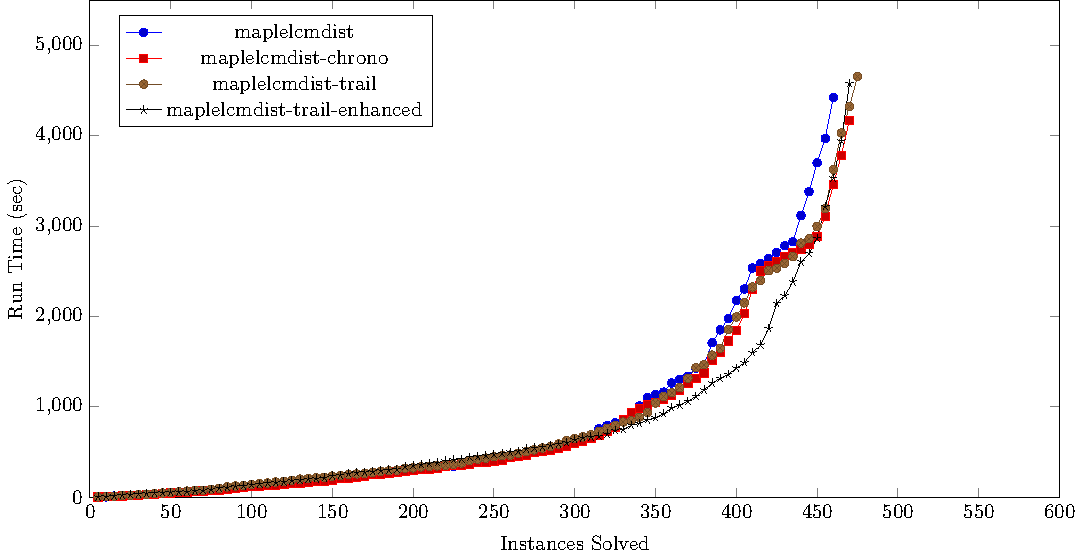
\includegraphics[scale=0.8]{cactus_maple2.pdf}\caption{\small{Comparison of run times for versions of MapleSAT. maplelcmdist is from the 2017 SAT Competition, maplelecmdist-chrono is with chronological backtracking (2018 SAT Competition), maplelcmdist-trail is with the first version of trail saving, maplelcmdist-trail-enhanced is with trail saving and all enhancements added.}}\end{figure}
\begin{figure}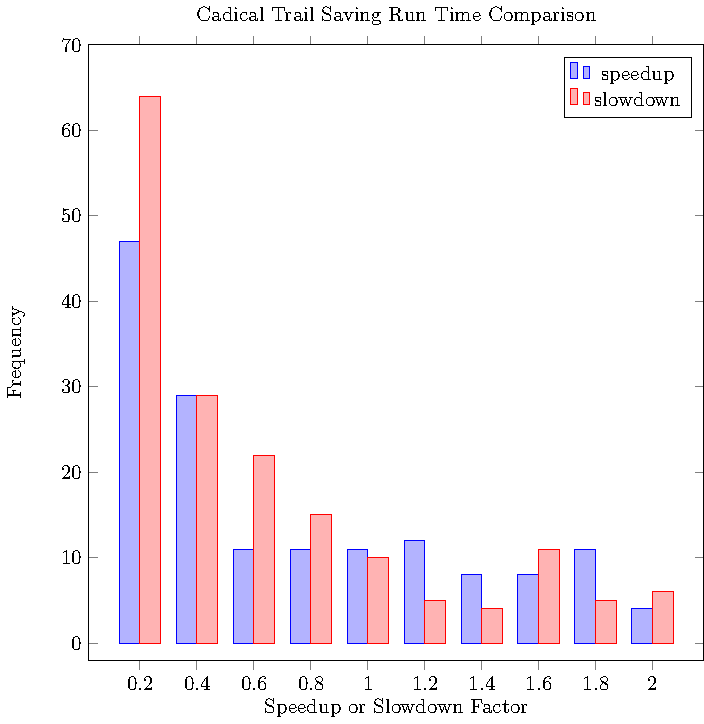
\includegraphics[scale=0.8]{test.pdf}\caption{}\end{figure}
\begin{figure}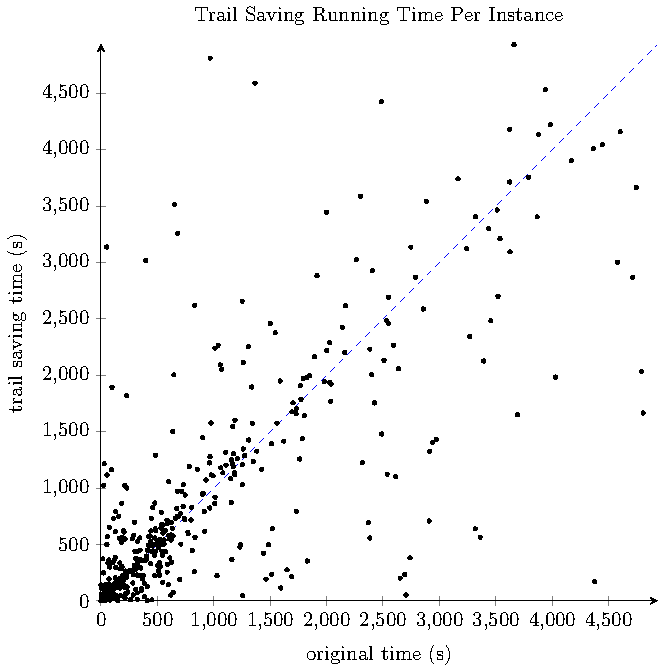
\includegraphics[scale=0.8]{test2.pdf}\caption{}\end{figure}
\iffalse
\begin{figure}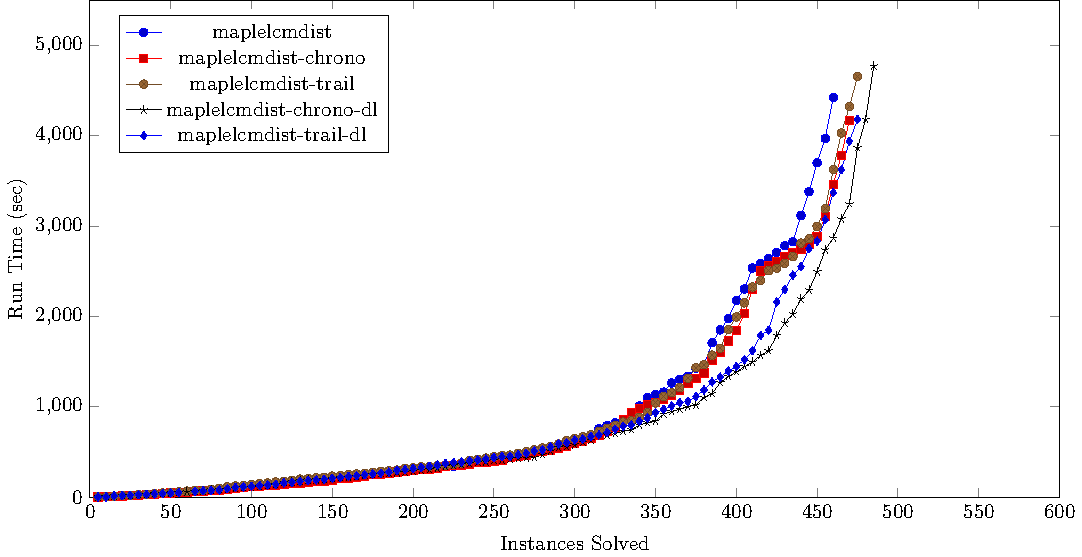
\includegraphics[scale=0.8]{cactus_maple.pdf}\caption{\small{Comparison of run times for versions of MapleSAT. maplelcmdist is from the 2017 SAT Competition, maplelecmdist-chrono is with chronological backtracking (2018 SAT Competition), maplelcmdist-trail is with the first version of trail saving, maplelcmdist-chrono-dl is with chronological backtracking and duplicate learnts (2019 SAT Competition), maplelcmdist-trail-dl is with trail saving and duplicate learnts}}\end{figure}
\fi
\clearpage

\iffalse
\begin{figure}[t]
\begin{center}
    \fss{9pt}{10pt}
	\setlength\tabcolsep{1pt}
	\begin{tabular}{| p{4.2cm} | c | c | c | c | c | c | c | c |}
	  \hline
	  & \multicolumn{4}{|c|}{Total} & \multicolumn{2}{|c|}{Unweighted} & \multicolumn{2}{|c|}{Weighted} \\ \hline
	  & MaxHS & +/- & \hspace{1pt} RC2 \hspace{1pt} & +/- & MaxHS & \hspace{1pt} RC2 \hspace{1pt} & MaxHS & \hspace{1pt} RC2 \hspace{1pt} \\ \hline
	  original & 6052 & 0/0 & 6030 & 0/0 & 3940 & 3993 & 2112 & 2037 \\ \hline
	  enqueue assumptions as set & 6131 & 114/35 & 6081 & \hspace{0.5pt} 99/48 \hspace{0.5pt} & 3995 & 4032 & 2136 & 2049 \\ \hline
	  enqueue assumptions as set + \newline save literals after learnt units & 6136 & 120/36 & 6079 & \hspace{0.5pt} 95/46 \hspace{0.5pt} & 3991 & 4030 & 2145 & 2049 \\ \hline
	  enqueue assumptions as set + \newline save literals after learnt units + \newline save literals from last invocation & 6138 & 115/29 & 6080 & \hspace{0.5pt} 92/42 \hspace{0.5pt} & 3989 & 4030 & 2149 & 2050 \\ \hline
	\end{tabular}
\end{center}
\caption{Number of \maxsat instances solved by MaxHS and RC2 using
  different extensions of the underlying \sat solver. The +/- column shows
  the number of instances gained/lost vs the original.}
\label{fig:nsolved}
\end{figure}
\fi

\section{Conclusion}

\bibliography{ref}{}
\bibliographystyle{splncs04}
\end{document}
